
%(BEGIN_QUESTION)
% Copyright 2015, Tony R. Kuphaldt, released under the Creative Commons Attribution License (v 1.0)
% This means you may do almost anything with this work of mine, so long as you give me proper credit

Sketch phasor diagrams of both the input phase voltages ($V_A$, $V_B$, and $V_C$) and the output phase voltages ($V_X$, $V_Y$, and $V_Z$) for this Wye-Delta transformer bank powering a resistive load, assuming 1:1 transformer turns ratios, an input line voltage of 2400 volts, an A-B-C phase sequence, and using phase A as the reference voltage (0 degree phase angle with reference to ground):

$$\includegraphics[width=15.5cm]{i00820x01.eps}$$

{\it Hint: since all transformers have a 1:1 turns ratio, the secondary voltage must be identical to the primary voltage for each one.  This means the phasor representing a transformer's secondary winding voltage must be exactly the same length and have exactly the same angle as the phasor representing that same transformer's primary voltage.  Treat each phasor as a line segment you are free to move around so long as you do not alter its length or direction, and you can see how they ``stack up'' onto each other according to how the windings are electrically connected to form a complete phasor diagram.}

\underbar{file i00820}
%(END_QUESTION)





%(BEGIN_ANSWER)

If ``A'' is the reference phasor and the sequence is A-B-C, it means phase B must lag 120 degrees behind phase A, and phase C must lag 120 degrees behind phase B (same as leading phase A by 120 degrees).  Thus:

$$V_A = 1385.6 \hbox{ V} \angle 0^o \hskip 20pt V_B = 1385.6 \hbox{ V} \angle -120^o \hskip 20pt V_C = 1385.6 \hbox{ V} \angle 120^o$$

$$\includegraphics[width=15.5cm]{i00820x02.eps}$$

Given the 1:1 transformer turns ratios, the Delta-connected line voltage must be the same as the Wye-connected phase voltage (1385.6 VAC).  Measuring $V_X$, $V_Y$, and $V_Z$ with reference to ground means these are phase voltages to the 1385.6 volt line voltage, and therefore each of them must have a value of 800 volts (1385.6 volts $\div$ $\sqrt{3}$).

Judging by the secondary phasor diagram, $V_Z$ must have a phase angle of 90$^{o}$ because that phasor points straight up.  The other two secondary phasors are, of course, shifted 120$^{o}$ in either direction from each other, which leads to the following results:

$$V_X = 800 \hbox{ V} \angle -30^o \hskip 20pt V_Y = 800 \hbox{ V} \angle -150^o \hskip 20pt V_Z = 800 \hbox{ V} \angle 90^o$$

%(END_ANSWER)





%(BEGIN_NOTES)

Phasor $V_{XY}$ must point in the same direction as phasor $V_A$ because they are of the same transformer, with 0 degrees of shift (ideally) between primary and secondary windings.  Ditto for $V_{YZ}$ and $V_B$, and for $V_{ZX}$ and $V_C$.  All I did to create the triangle for the secondary phasor diagram was to copy the phasors of the primary diagram and place them tip-to-tail as dictated by the wiring connections between secondary windings.  Neither the length nor the angle of any phasor was altered.

\vskip 10pt

Incidentally, this 30 degree phase shift is in accordance with the IEEE standard for power transformers: that the lower-voltage side should lag 30 degrees behind the higher-voltage side when the connection is Wye-Delta or Delta-Wye.

%INDEX% Electronics review: AC transformer circuit
%INDEX% Electronics review, phasor expressions of circuit quantities
%INDEX% Electronics review, 3-phase transformer bank phase shift calculations

%(END_NOTES)


